\documentclass{article}
\usepackage{tikz}
\usetikzlibrary{arrows.meta, decorations.pathreplacing, positioning, quotes}

\begin{document}

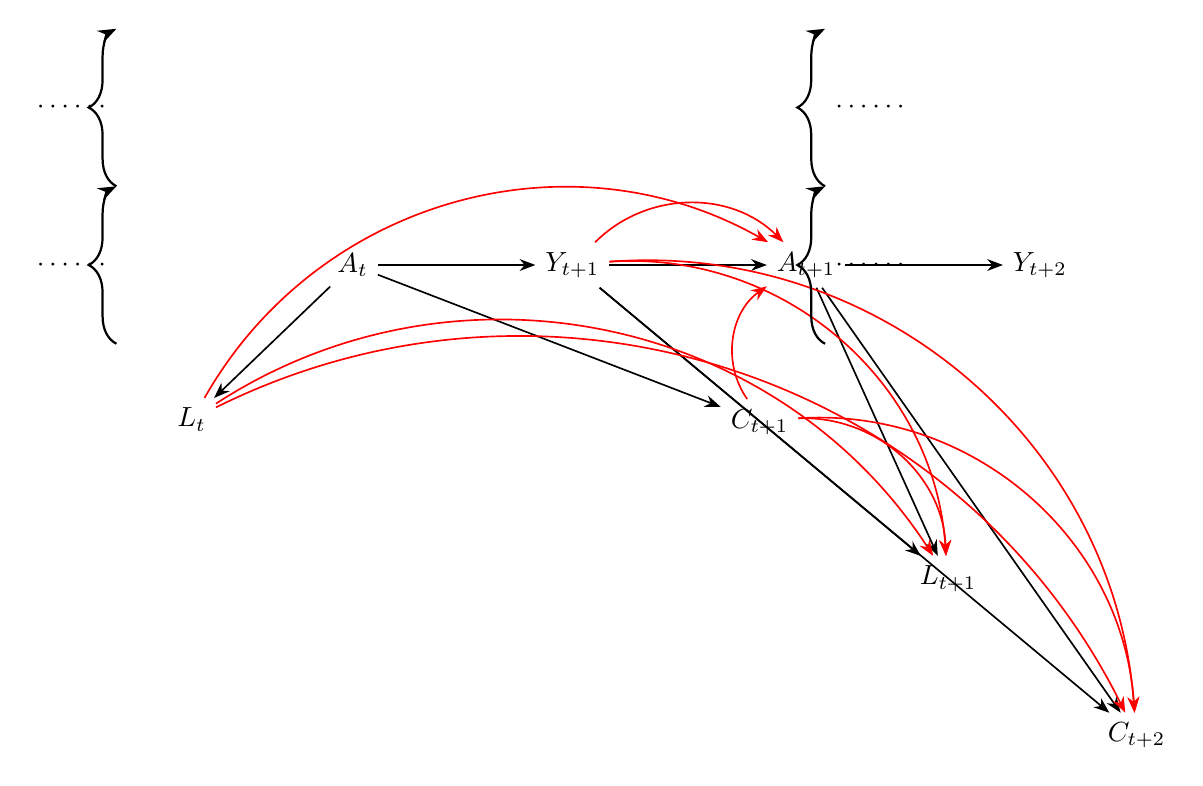
\begin{tikzpicture}[->, >=Stealth, auto, semithick, node distance=2cm]
    \node (A) {$A_t$};
    \node[below left=of A] (L) {$L_t$};
    \node[right=of A] (Y) {$Y_{t+1}$};
    \node[right=of Y] (A1) {$A_{t+1}$};
    \node[right=of A1] (Y1) {$Y_{t+2}$};
    \node[below right=of Y] (C) {$C_{t+1}$};
    \node[below right=of C] (L1) {$L_{t+1}$};
    \node[below right=of L1] (C1) {$C_{t+2}$};

    \draw[->] (A) -- (Y);
    \draw[->] (A) -- (C);
    \draw[->] (A) -- (L);
    \draw[->] (Y) -- (A1);
    \draw[->] (Y) -- (C1);
    \draw[->] (Y) -- (L1);
    \draw[->] (A1) -- (Y1);
    \draw[->] (A1) -- (C1);
    \draw[->] (A1) -- (L1);

    \draw[red, ->] (Y) to[bend left=45] (A1);
    \draw[red, ->] (Y) to[bend left=45] (C1);
    \draw[red, ->] (Y) to[bend left=45] (L1);
    \draw[red, ->] (C) to[bend left=45] (A1);
    \draw[red, ->] (C) to[bend left=45] (C1);
    \draw[red, ->] (C) to[bend left=45] (L1);
    \draw[red, ->] (L) to[bend left=45] (A1);
    \draw[red, ->] (L) to[bend left=45] (C1);
    \draw[red, ->] (L) to[bend left=45] (L1);

    \draw[decorate, decoration={brace, amplitude=10pt}, thick] (-3,-1) -- (-3,1) node[midway, left] {$\cdots\cdots$};
    \draw[decorate, decoration={brace, amplitude=10pt}, thick] (-3,1) -- (-3,3) node[midway, left] {$\cdots\cdots$};
    \draw[decorate, decoration={brace, amplitude=10pt}, thick] (6,-1) -- (6,1) node[midway, right] {$\cdots\cdots$};
    \draw[decorate, decoration={brace, amplitude=10pt}, thick] (6,1) -- (6,3) node[midway, right] {$\cdots\cdots$};
\end{tikzpicture}

\end{document}